\chapter{Enabling technologies}
\label{chap:state_of_the_art}

\begin{chapterintro}

In this chapter, a brief introduction of the state of the art for conversational agents and Question Answering is presented. Likewise, we will take a short look at some Linked Open Data systems, and the ways to recover data for them.


\end{chapterintro}

\cleardoublepage

\section{Overview}

Conversational agents, presented in section \ref{sec:conv_agents} are systems that allow an user to interact with using natural language, the same way they will interact will another humar being. This is achieved by using engines that analyse the user input, process it, and provide the best possible answer given the knowledge of the system.

Question answering systems work in a similar way, but rather than provide a response in natural language, they present the user the resource where the answer to their question is located, usually by translating the question to a specialised query for a given database.

The aforementioned database is usually a Linked Open Data System. This systems allow the publication of Semantic data, connecting it to the world and making therefore easily accesible and linkable.

Finally, we will study the way of populating the system, using web scrapping techniques in order to recover the information when it is not presented as Linked Open Data.


\section{Conversational Agents}
\label{sec:conv_agents}

In this section we will discuss the evolution of conversational engines, and discuss a few of the techniques and technologies utilized implementing them. We will provide a small overview to \ac{AIML} and some engines implemented with it, as well as other engines to finalise with a small description of ChatScript.

One of the starting points when studying conversational agents is A.L.I.C.E. an free natural language artificial intelligence chat robot that utilizes AIML for creating responses based on the user input to the system. ALICE won the 2000, 2001, and 2004 Loebner prizes, becoming a starting point while developing conversational agents. It makes use of the pattern-matching ability of AIML, with 120.000 patterns that can either trigger a response o redirect the input to another pattern. ALICE was inspired by Eliza, on the first examples of natural language processing using simple patterns, written at MIT by Joseph Weizenbaum between 1964 and 1966.

Along with ALICE, a number of other AIML conversational agents have been presented to the Loebner contest, by different authors, usually getting good results, like Mitsuku, by Steve Worswick, who won the 2013 edition of the contest, and was among the 4 finalists in 2014, three of them using AIML. Another example of an AIML bot is Izar, by Brian Rigsby, who achieved second place in the 2014 contest

The winner of the 2010, 2011 and 2014 contests was Bruce WillCox, using different chatbots, all of them written in ChatScript. Chatscript was presented in 2010, written in C++, and later released as Open Source. Whilst AIML aims to pattern-match words, ChatScript claims to match in a general meaning basis, focusing on detecting equivalence and paying heavy attention to sets of words and canonical representation, and providing a simple way of storing user data, in a machine readable format.

\subsection{\ac{AIML}}

\ac{AIML}~\cite{aimlprimer} is a widely use XML dialect for creating conversational language. It was developed between 1995 and 2002 by Richard S. Wallace and the free software community, and has remained relevant to this date, including the draft for a major upgrade, AIML 2.0, released in the early 2013, and currently being working on. The original version of AIML had seven design goals, stated in its primer:
\begin{enumerate}%[topsep=0pt,itemsep=-1ex,partopsep=1ex,parsep=1ex]
  \item Shall be easy to learn.
  \item Shall encode the miniaml concept set necessary to enable a stimulus-response knowledge system modelled on that of the original A.L.I.C.E.
  \item Shall be compatible with XML.
  \item It shall be easy to write programs that process AIML documents.
  \item \ac{AIML} objects should be human-legible and reasonably clear.
  \item The design of \ac{AIML} shall be formal and concise.
  \item \ac{AIML} shall not incorporate dependencies upon any other language.
\end{enumerate}

There are more than twenty tags for the AIML language~\cite{aliceaiml}, but the most important units are \emph{aiml}, the tag that defines a document as \ac{AIML}, \emph{category} marking a ``unit of knowledge'' in the bot's knowledge base, \emph{pattern} contains a simple pattern that will be compared with the user input, and \emph{template} containing the response to a user input.

\begin{center} 
  \begin{lstlisting}[language=XML, captionpos=b, caption=Example AIML code, label=listing:exampleaiml]   
    <category>
        <pattern> WHO ARE YOU </pattern>
        <template>I am a bot </pattern>
    <category>
 \end{lstlisting}
\end{center}
The free A.L.I.C.E. \ac{AIML}~\footnote{\url{http://www.alicebot.org/downloads/}} includes a knowledge base of 41.000 categories, and can be used as a base for others bots.

\subsubsection{\ac{AIML} 2.0}

In January 2013 the ALICE A.I. Foundation released a draft specification for a major update for \ac{AIML}~\footnote{\url{http://alicebot.blogspot.com.es/2013/01/aiml-20-draft-specification-released.html}}, aiming to provide new features while trying to keep \ac{AIML} as simple as possible. \ac{AIML} 2.0 combines Pandorabots extensions to the language, \ac{OoB} tags and a collection of new features. The full list of new features can be found in the Working Draft~\cite{aiml20draft}, some of the more relevant are:

\begin{itemize}%[topsep=0pt,itemsep=-1ex,partopsep=1ex,parsep=1ex]
  \item Zero+ wildcards, allowing to match zero or more words
  \item Setting matching priority for certain words.
  \item Loops.
  \item \ac{OoB} tags.
  \item Local variables.
\end{itemize}

\subsubsection{\ac{AIML} implementations}

\ac{AIML} has been implemented in multiple languages, including Java, Python, PHP or C++. Some of those implementations are listed in the ALICE downloads page~\footnote{\url{http://www.alicebot.org/downloads/programs.html}}, and we will briefly describe some of them bellow:

\begin{enumerate}
 \item \textbf{Program D} is a Java implementation, open source, implementing the \ac{AIML} specification. It supports multiple bots per instance, and provides multiple ways to interfaces to interact with the service, providing a J2EE release allowing deployment as a webservice. However, the development of this project has been stagnated for years, with its last release in 2006.
 \item \textbf{ChatterBean} is another Java implementation, aiming to be \ac{AIML} 1.0.1 compliant, using a JavaBeans plugin architecture, and released under a GPL license. However, the last version was released on 2006 and the development since then seems to have stopped.
 \item \textbf{Program O}, written in PHP with MySQL, is an \ac{AIML} engine with a web interface providing a number of remarkable features, including an administration panel, with configuration, teaching an testing interfaces. It stores the \ac{AIML} files in a MySQl database in order to improve its performance, and can assign different personalities to each bot. It is under active development by Ellizabeth Perreau and Dave Morton, with it latest version released in May 2014. 
\end{enumerate}


\begin{figure}[!htbp]
    \centering
    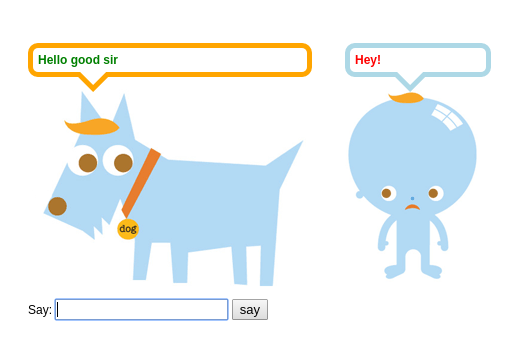
\includegraphics[width=0.9\textwidth]{img/screens/programo.png}
    \caption{Demo interface for Program-O.}
    \label{fig:programo1}
\end{figure}


\subsection{ChatScript}
\label{subsec:chatscript}

ChatScript, written in C++ by Bruce Willcox, is a chatbot engine aiming to overcome the limitations of \ac{AIML}, by providing pattern matching on general meaning rather than particular words. It was originally created for Avatar Reality, a start-up company that wanted to create a virtual world called Blue Mars~\cite{Wilcox2010suzzete}, and it was eventually released as open source as per the requirements for the Loebner prize.

Since then, ChatScript has been updating and introducing improvements, up to version 5.4~\cite{ChatScriptSourceForge}. Some of the features in ChatScript include:
\begin{itemize}
 \item Efficient, easily readable output rules
 \item Zero-length wildcards
 \item Concise pattern matching through the use of concepts
 \item Built-in data covering multiple subjects and topics
\end{itemize}

By matching in meaning, ChatScript claims to be able to provide a better user experience than \ac{AIML}, with a much smaller rule set, improving maintainability and ease to modify the bot whenever necessary. More details on ChatScript are provided in section ~\ref{subsec:chatscript}.

\subsubsection{Basic syntax, topics and rules}

In Chatscript, rules are grouped in topics, and stored in ``.top'' files, allowing the designer to map the point of the conversation, therefore making a better response for the user. And example topic file can be found in listing~\ref{listing:exampletop}. In this example, the topic will be triggered when the user writes an input containing the words ``name'', ``here'', ``what'', or any other word specified in the system dictionaries ``emogoodbye'', ``emohello'' or ``emohowzit''. Then, it will attempt to match the user input with the patterns ``what is your name'' and ``what ~be''. If no pattern matches, it will output the gambit ``Have you been here before?''.

\begin{center} 
  \begin{lstlisting}[language={}, captionpos=b, caption=Example topic file, label=listing:exampletop]   
    topic: ~INTRODUCTIONS (~emogoodbye ~emohello ~emohowzit name here what )
    
    #!x issued only once, then erased
    t: Have you been here before?
    
    #! what is your name 
    u: ( what is your name ) 
        My name is Harry.
        
    #! what are you ?
    ?: ( what ~be )
        I am a bot. Are you also a bot?
        a: (~no)
            Oh, a human... How can I help you?
  \end{lstlisting}
\end{center}

In this simple example, we find some of ChatScript syntaxes elements. We can see responders, gambits and rejoinders, as well as the use of topics and concepts. These are part of ChatScript rules structure, but there are some more elements not shown here. A slightly more comprehensive list is as follows:
\begin{itemize}
 \item \textbf{Input matching:} The pattern can start with either ``s:'', ``?:'' or ``u:'', indicating they are supposed to respond to statements, questions or both. The parenthesis then indicate the pattern itself, which can have multiple elements:
    \subitem \emph{General words:} A simple word to look for on the sentence. ChatScript handles plurals and verb conjugations.
    \subitem \emph{Concepts:} Starting with \~ , a concept is a set of words with a common general meaning.
    \subitem \emph{Wildcards:} Allowing to match any word, or using a cardinal, can specify the number of words to match with the wildcard.
    \subitem \emph{Start and end of sentence:} Using > and <, its possible to indicate whether the pattern should match the start or the end of the sentence.
    \subitem \emph{Variables: } Starting the pattern element, whether is a wildcard, a concept or a word, using ``\_'', will store the matched word in a variable for future use, be it in the response or somewhere else.
  \item \textbf{Gambit:} Lines starting with ``t:'' indicate a gambit, that will be triggered when the bot cannot find an appropriate response.
  \item \textbf{Bot Response:} Immediately after the pattern, the following lines until the next chatscript syntax element indicate how the bot response is formed.
  \item \textbf{Variables:} Not shown in the previous example, any word starting with ``\$'' is a global variable, and can be assigned a value that will be remembered for the user. If the variable starts with ``\$\$'', the variable will be local, only lasting until the end of the current answer.
  \item \textbf{Rejoinders} Starting with single letters from ``a:'' through ``q:'' to indicate nesting depth, this indicate patterns that will trigger when the user responds to a specific bot output.
  \item \textbf{Concepts:} Sets of word with a specific meaning, when referring to a concept in a pattern, it will match if any word in the set matches the input. ChatScript includes a large set of concepts by default, but the user can define its own sets.
  \item \textbf{Topics:} rules are grouped in topics. Rules inside the topic will only be tested against the input when the input itself contains any of the words specified while defining the topic.
\end{itemize}

A more detailed approach to ChatScript rules, matching and functions can be found in its documentation\footnote{\url{http://sourceforge.net/projects/chatscript/files/}}.

\subsubsection{Deploying a bot with ChatScript}

By default, ChatScript can be run in local or server mode. Local mode allows for direct interaction from the command line, using the standard input and output to communicate with the user. This mode is specially usefull for debugging the rules when developing bots, since it gives access to debugging commands build with the system.

For production environments, ChatScript can be run in server mode, where it listens it offers a TCP interface. This interface will receive messages containing the bot name, the user name and the user input, and return the bot response for the given input.

\section{Question Answering Systems}
\label{sec:qa_sys}

\ac{QA} is a discipline concerned with automatically provide answers to questions presented in natural language, using a number of different approaches in order to process the question into a query the system can understand, and, therefore, answer.

In general, we can differentiate six major general approaches~\cite{unger2014an}:

\begin{itemize}
  \item \textbf{Controlled natural languages:} The system only takes into account a well-defined subset of a given natural language that can be unambiguously interpreted.
  \item \textbf{Formal grammars processing:} Relaying on linguistics to assign syntactic and semantic representations to lexical units, as well as compositional semantics, this systems compute a representation of the question. Two examples of this systems could be ORAKEL~\cite{cimiano2008towards} and Pythia~\cite{unger2011pythia}
  \item \textbf{Mapping linguistics to semantic structures:} Systems designed under this principle rely on a measure of similarity between elements in the query and the predicates, subjects or objects in the knowledge base. PowerAqua~\cite{lopez2011poweraqua} and Aqualog~\cite{lopez2007aqualog} are two examples of this approach.
  \item \textbf{Template-based:} Taking two stages, this approach first construct a query based on the linguistic analysis of the input question, and the matchs the expressions in the question with elements from the dataset. TBSL~\cite{unger2012template} implements this approach.
  \item \textbf{Graph exploration:} This approach maps elements of the question to entities in the knowledge base, and proceeds navigation from these pivot elements to navigate the graph, seeking to connect the entities to yield a connected query. This example is taken by the TREO~\cite{freitas2011querying} system
  \item \textbf{Machine learning:} question answering has been considered a machine learning problem, with either models for joint query interpretation and response ranking, aiming at learning semantic parsers given a knowledge base and a set of questions and answers, or systems with an algorithm for matching natural language expressions and ontology concepts, as well as an algorithm for storing matches in a parse lexicon.
\end{itemize}

%\emph{\textcolor{red}{Shortly describe the exampe systems?}}

To the aforementioned systems, we have to add another one: IBM Watson's DeepQA. Designed to be a contestant in the Jeopardy! quiz show, the DeepQA system had multiple information sources, the DeepQA system focused on extracting and scoring evidence from unstructured data, although it also used structured an semantic data sources. It was build as a massively probabilistic evidence-based architecture using more than 100 different techniques for analysing natural language. It was build using Apache UIMA\footnote{\url{http://uima.apache.org/}}, an Unstructured Information Management system.

%\emph{\textcolor{red}{Add figure or list with the structure?}}

\section{Linked Data Systems}
\label{sec:linkd_sys}

Linked Data consists in a set of rules about publishing data in the web so it can be interlinked and accessed using semantic queries. The term was first used by Tim Berners-Lee while talking about the Semantic Web project. Additionally, Linked Open Data is an extension of the Linked Data concept, requiring that the data provided is open content.

\begin{figure}[!htbp]
  \begin{minipage}{\linewidth}
    \centering
    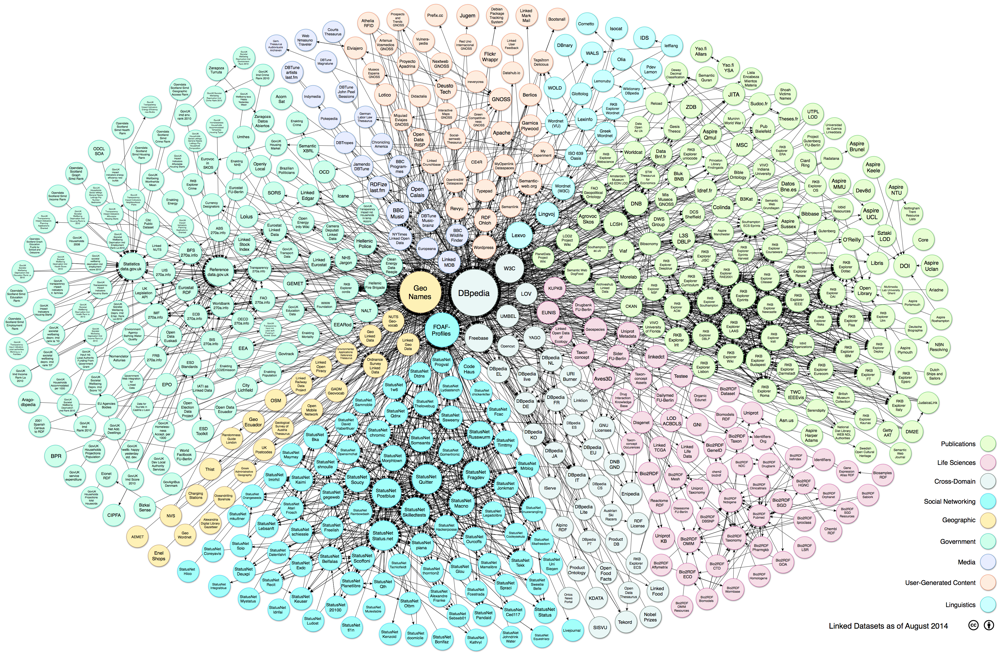
\includegraphics[width=\textwidth]{img/enabling/lod-cloud.png}
    \caption[Linked Open Data cloud]{%
      Linked Open Data cloud%
      \footnote{\url{http://lod-cloud.net/}}%
      }
    \label{fig:lodcloud}
  \end{minipage}
\end{figure}

There are a number of Linked Data Systems publicly available to the public, as long as multiple projects allowing to deploy your own linked data services. Some of them are described in the next sections. 

\subsection{Apache Lucene and Solr}
\label{sec:statesolr}

Not considered Linked Data Systems on its own, Apache Lucene~\footnote{\url{http://lucene.apache.org/}} is a high-performance full-featured text search engine, that can be used as the foundation of many systems. Apache Solr is built on top of Lucene, providing distributed indexing, replication and querying, with multiple features and functionalities~\footnote{\url{http://lucene.apache.org/solr/}}:

\begin{itemize}%[topsep=0pt,itemsep=-1ex,partopsep=1ex,parsep=1ex]
  \item Full-text search, with powerful matching capabilities, powered by Lucene.
  \item Optimized for High Volume traffic.
  \item Standards Based Open interfaces, including json, xml and http.
  \item Comprehensive Administration Interfaces, making it easy to handle Solr instances.
  \item Easy Monitoring, publishing relevant data via JMX
  \item Highly scalable and Fault tolerant, using Apache ZooKeeper, is easy to scale and distribute the load.
\end{itemize}

Apache Solr is used as a base in many other systems, including some of the described in the following sections, and can also be used as a \ac{QA} system of its own\cite{ingersoll2013taming}.

\begin{figure}[!htbp]
    \centering
    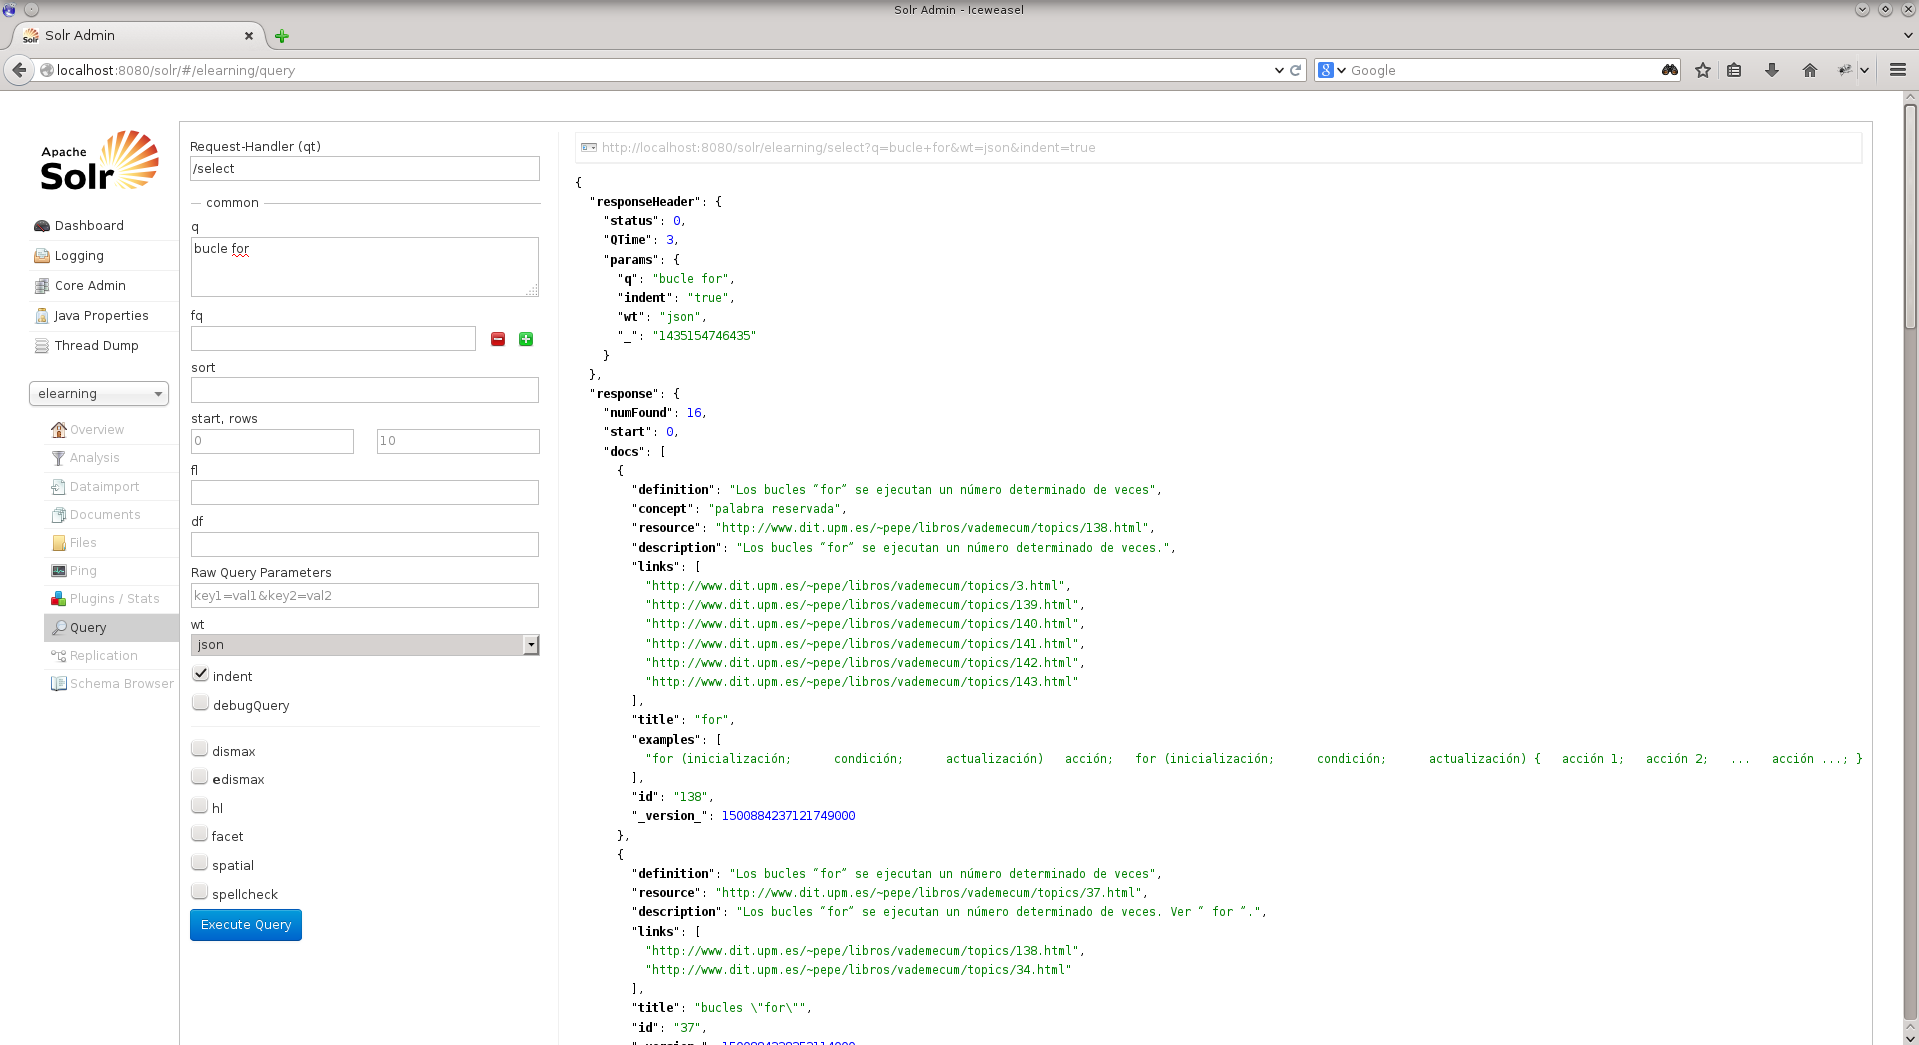
\includegraphics[width=0.9\textwidth]{img/screens/solr-interface.png}
    \caption{Web interface for Solr queries.}
    \label{fig:solr1}
\end{figure}

% Add stanbol here?

\subsection{Linked Media Framework and Apache Marmotta}

Started as the Linked Media Framework\footnote{\url{https://bitbucket.org/srfgkmt/lmf/}}, this project aimed to provide an easy to setup server to offer linked media management, publishing linked data and allowing interactions with it. \ac{LMF} is built in modules, some of them optional, allowing the extension of the functionalities in the Linked Media Server. Some of the implemented modules are:

\begin{itemize}%[topsep=0pt,itemsep=-1ex,partopsep=1ex,parsep=1ex]
  \item \ac{LMF} Semantic Search allowing for a search service on top of Apache Solr. 
  \item \ac{LMF} Stanbol Integration, using Apache Stanbol for content analysis and interlinking.
  \item \ac{LMF} SKOS editor, to manage SKOS thesauruses imported in the Linked Media Server.
\end{itemize}

The core functionalities of \ac{LMF} where set aside to incubate Apache Marmotta, an Open Platform for Linked Data within the Apache Software Foundation~\footnote{\url{http://www.apache.org/}} aiming to provide an implementation for Linked Data that can be used to both publish Linked Data and build custom applications for Linked Data.

\subsection{Fuseki and Apache Jena}

Fuseki, build using Apache Jena\footnote{\url{http://jena.apache.org}}, is a \ac{SPARQL} server that provides a REST-style interface for \ac{SPARQL} queries. Its build using Apache Jena, an open source Semantic Web framework for Java. Apache Jena provides an API to extract data and write it to \ac{RDF} graphs, that are represented as an abstract model. A model can be sourced with data from files, databases, URLs or any combination of them. It also provides support for \ac{OWL}, and comes with several internal reasoners, as well as having support to use the Pellet\footnote{\url{https://www.w3.org/2001/sw/wiki/Pellet}} reasoner for \ac{OWL}

% Apache Marmotta / LMF
% DBpedia / virtuoso?
% Apache UIMA ?
% Apache Lucene / Solr / Stanbol ? 
% Terrier ? 



\section{Information retrieval}

The amount of information available in the web has grown exponentially over the last years, with standards such as Linked Data helping exchange data among heterogeneous systems. However, many times these standards are not used, and so it becomes necessary to recover and convert the data into compatible formats. There are multiple frameworks capable of crawling the web and recovering the relevant pieces of information, but we will focus here in Scrappy, a framework in ruby that allows extracting information from web pages and producing RDF data, and Scrapy, a python tool that allows extracting data from websites into any format, with powerful capabilities.

% Scrappy and scrapy

\subsection{Scrappy}
\label{subsec:scrappy}

Scrappy\cite{villamor13} is a ruby framework with multiple functionalities, including web and REST interface, storing the scrapped data in a RDF repository, and outputing in multiple formats. For our system, we will discuss the web scrapping and RDF output capabilities.

To recover data from a web page, Scrappy utilizes an ontology\footnote{http://www.gsi.dit.upm.es/ontologies/scraping/} to define the mapping between the web data and the semantic web resources. An example extractor can be found in listing \ref{listing:examplescrappy} will take the link to the GSI's staff page and return a foaf object with the name of each member. As seen in the extractor, it matches CSS elements in the page to semantic properties. Although not shown in this particular example, it can also use Xpath and regular expressions as selectors.

\begin{center} 
  \begin{lstlisting}[language={}, captionpos=b, caption=Example extractor, label=listing:examplescrappy]   
dc: http://purl.org/dc/elements/1.1/
rdf: http://www.w3.org/1999/02/22-rdf-syntax-ns#
sioc: http://rdfs.org/sioc/ns#
sc: http://www.gsi.dit.upm.es/ontologies/scraping.rdf#

_:gsipeople:
  rdf:type: sc:Fragment
  sc:type: foaf:Person
  sc:selector:
    *:
      rdf:type: sc:UriPatternSelector
      rdf:value: "http://www.gsi.dit.upm.es/index.php?option=com_jresearch&view=staff&layout=positions"
  sc:identifier:
    *:
      rdf:type: sc:BaseUriSelector
  sc:subfragment:
    *:
      sc:type: foaf:Person
      sc:selector:
        *:
          rdf:type: sc:CssSelector
          rdf:value: ".jrperson"
      sc:identifier:
        *:
          rdf:type: sc:CssSelector
          rdf:value: "a"
          sc:attribute: "href"
      sc:subfragment:
        *:
          sc:type: rdf:Literal
          sc:relation: foaf:givenName
          sc:selector:
            *:
              rdf:type: sc:CssSelector
              rdf:value: "a"
  \end{lstlisting}
\end{center}

An example of data generated with that extractor is shown in listing ~\ref{listing:examplerdf}. It can be seen how the elements matched in the extractor have been converted into properties. 

\begin{center}
  \lstinputlisting[language=XML, captionpos=b, caption=Example person extracted with Scrappy, label=listing:examplerdf]{code/enabling/person.rdf}
\end{center}

Using the appropriate selectors, scrappy can follow the links on a page, automating the scraping of big web sites, and converting all the data into RDF, N-Triples or JSON-LD.

\subsection{Scrapy}

Scrapy\footnote{\url{http://scrapy.org/}} is a fast high level web crawling framework, used to extract structured data from websites. It is written in python, and by default outputs data to json, although it accepts custom exporters, giving the user the ability to export into any format it requires.

The crawlers are python classes that extend the Spider class in scrapy.

\definecolor{Strings}{rgb}{0,0.63,0}
\begin{center}
  \lstinputlisting[language=Python, stringstyle=\color{Strings}, captionpos=b, caption=Example scrapy spider, label=listing:examplescrapy]{code/enabling/scrapy.py}
\end{center}

Listing \ref{listing:examplescrapy} shows part of a scrapy spider that will return a json object containing the url of the scrapped page, as well as the title, alternative and concept fields scrapped from the document.

\section{Web technologies}

% Talk about all-web movement? JavaScript & JQuery? 

% This is mostly bullshit. Rewrite it.

Known simply as ``The web'', the World Wide Web is an information system where hypertext documents are accessed via the internet. First proposed by Tim Berners Lee in 1989\cite{berners1989information}, it has grown to be used by two in five people around the world\footnote{\url{http://webfoundation.org/about/vision/history-of-the-web/}}.

The technologies used in web services can be divided in Client technologies, executed in the user's computer, and Server technologies, executed in the server side of the service. We will provide a short description of some of the technologies available for each side, focussing on those used in this project.

\subsection{Client technologies}

Web browsers are usually responsible for running the code of a website. Usually, that code consists on CSS, HTML and JavaScript files, that are interpreted by the browser to present the page, and respond to the user actions.

\begin{itemize}
 \item \textbf{HTML}: or \emph{HyperText Markup Language} is the standard markup language used to create web pages. It consists on a collection of pairs of tags that identify the different elements on a page, describing the structure of the page. It can also include images and other objects, allowing for complex user interaction.
\item \textbf{CSS}: for \emph{Cascading Style Sheets} is a style sheet language, used mostly to describe the look and formatting of documents written in a markup language such as HTML. It is designed to allow separation of content from document presentation, providing more flexibility and control of the presentation, while also improving accessibility.
 \item \textbf{JavaScript} is a programming language used to run scripts to interact with the user inside the browser window. Along with JavaScript, its most used library\footnote{\url{http://libscore.com/\#libs}} is jQuery, which is designed to simplify many of the usual tasks performed with JavaScript.
\end{itemize}

This technologies are often used with Ajax (\emph{Asynchronous Javascript XML}), a group of web development techniques used to create asynchronous web applications. Using Ajax, web applications can interact with the server in the background, therefore not interfering with the behaviour and graphical display of the rest of the page.

% JS/jQuery, HTML5, CSS, etc

\subsection{Server technologies}

% HTTP Servers. Apache?

The interactions presented by the web client are the processed in the server side, usually communicating using HTTP. There are multiple applications capable of handling this interaction, known as http servers. Apache, NginX or Microsoft Windows Server\textregistered~are some of the most popular servers\footnote{\url{http://news.netcraft.com/archives/2015/05/19/may-2015-web-server-survey.html}}. 

For our service, we have used Apache\cite{apacheabout}, an Open Source HTTP-Server. First launched in 1995, it has continued development to this date, with version 2.4.12 being released on January 2015~\footnote{\url{http://httpd.apache.org/}}. It is currently developed and maintained by an open community of developers under the Apache Software Foundation, and made available in a wide variety of operating systems, including GNU/Linux and Microsoft Windows\textregistered. It features a module-based system, allowing the core functionality to be expanded by compiled modules. Some of the most popular modules include:

\begin{itemize}%[topsep=0pt,itemsep=-1ex,partopsep=1ex,parsep=1ex]
 \item \textbf{mod\_php} Enabling the use php to execute server side code, this module can be found in many Apache installations, allowing the deployment of services like WordPress or Joomla.
 \item \textbf{mod\_auth\_basic} Handling basic user authentication, this module allows the server administrator to block sections of the server from being accessed by the general public.
 \item \textbf{mod\_proxy} Allows the use of Apache as a proxy, masking other services behind it.
\end{itemize}

Over the last few years, there has been an important trend in the use of evented web technologies, a vision of the traditional web APIs complemented with other APIs that produce events, and provide with a callback mechanism, make the Web more like a giant network. Node.js\footnote{\url{https://nodejs.org/}} is one of the most popular environments to build this kind of applications.

\subsubsection{WSGI Servers in python}

\ac{WSGI} is a specification for simple interfaces between web servers and web applications for the python programming language. First defined in PEP 333\cite{pep0333}, and updated in PEP 3333\cite{pep3333}, it has been adopted as a standard for python web application development.

There are multiple implementations and frameworks of WSGI for python, some of the most popular are:

\begin{itemize}
 \item \textbf{Bottle} is a simple lightweight WSGI framework, focusing on simplicity. It is distributed as a single file module, with no other dependencies than the python standard library. However, it has capabilities to handle routing, easy access to web data such as cookies and http headers, and includes a built-in server for development. It also has support for templates, both with a built-in engine, and using external modules such as mako or jinja2.
 \item \textbf{Django} is a full-fledged python web framework, offering fast and scalable services, with multiple built-in options, such as security, administration tools. It is slightly higher level than other frameworks, and emphasizes reusability of components and plugins, as well as rapid development. % complete?
 \item \textbf{Flask}, a micro web application framework, based on the jinja2 template engine, and the Werkzeug WSGI toolkit. It focuses on providing a simple interface, whilst still providing multiple features such as RESTfull request dispatching, cookies and request handling and unicode support. It also includes native support for unit testing, as well as a development server and debugger. It also supports extensions for extra functionalities.
\end{itemize}

In our application, we have chose Apache as the gateway server, using mod\_wsgi, and Flask for the application itself. 
%\emph{\textcolor{red}{Give ``example'' apache config?}}

\section{Summary}

In this section, we have discussed the technologies related to the system we are developing.

First, we took a look at \emph{conversational agent} systems. We saw that AIML and its implementations provide a robust technology, that is still evolving despite its age. It has been widely used, and still has an large community and volume of users, and is working on the new AIML 2.0. We also considered ChatScript characteristics, with better performance and new language for writing bots, with a simpler syntax and features not present in AIML 1.

We then considered \emph{Question Answering} systems and its different approaches, also taking a look at some systems that use each approach.

As for \emph{Linked Data Systems}, we studied the concept of the Semantic Web and Linked Data, to then take a look at multiple systems used for it: Apache Solr, not a linked data system on its own, but used in many of them, the Linked Media Framework, a full fledged linked data servers built around Apache Marmotta, and Fuseki, a SPARQL server with reasoning capabilities build with Apache Jena.

After considering the Data indexing systems, we studied two \emph{Information Retrieval} tools: Scrappy, a ruby web crawler capable of exporting RDF documents from the data extracted from the web, and Scrapy, a python framework for web spiders, with support for multiple functionalities as well as allowing export of the data in personalised formats.

Finally, we took a quick look at \emph{web technologies}, both for client-side applications, as well as server side systems that would allow complex interactions with the user. We focussed specially in the server side, studying different implementations of WSGI modules for python, and considering their characteristics.
